\documentclass{standalone}
\usepackage{tikz}
\usepackage{ctex,siunitx}
\usepackage{tkz-euclide}
\usepackage{amsmath}
\usetikzlibrary{patterns, calc}
\usetikzlibrary {decorations.pathmorphing, decorations.pathreplacing, decorations.shapes,}
\begin{document}
\small
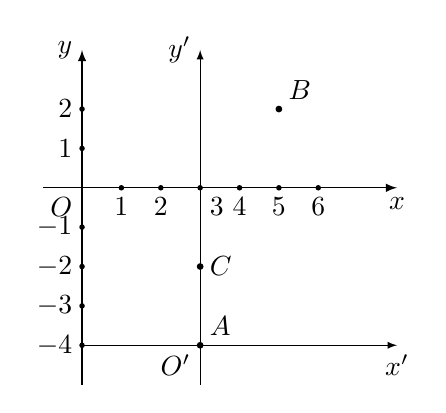
\begin{tikzpicture}[>=latex,scale=0.5]
  \draw[thin,->](-1,0)--(8,0)node[below]{$x$};
  \draw[thin,->](0,-5)--(0,3.5)node[left]{$y$};
  \draw[very thin,->](0,-4)--(8,-4)node[below]{$x'$};
  \draw[very thin,->](3,-5)--(3,3.5)node[left]{$y'$};
  \tkzDefPoints{0/0/O,3/-4/A,3/-4/O',5/2/B,3/-2/C}
  \foreach \x in {1,2,4,5,6} {\fill(\x,0)circle(2pt)node[below]{\x};}
  \foreach \x in {1,2,-4,-3,-2,-1} {\fill(0,\x)circle(2pt)node[left]{$\x$};}
  \fill(3,0)circle(2pt)node[below right]{3};
  \tkzDrawPoints[fill=black](A,B,C)
  \tkzLabelPoints[above right](A,B)
  \tkzLabelPoints[right](C)
  \tkzLabelPoints[below left](O,O')
\end{tikzpicture}
\end{document}